% Use the `standard` option to get 4x3 aspect ratio.
% Use the `noul` option if there is a conflict with the `\ul` command.
\documentclass{antclass}

\usepackage{amssymb}
\usepackage{amsmath}
\usepackage{verbatim}
\usepackage{graphicx}
\usepackage{listings}
\usepackage{xcolor}

% Code styling for better presentation
\definecolor{codegreen}{rgb}{0,0.6,0}
\definecolor{codegray}{rgb}{0.5,0.5,0.5}
\definecolor{codepurple}{rgb}{0.58,0,0.82}
\definecolor{backcolour}{rgb}{0.95,0.95,0.92}

\lstdefinestyle{cppstyle}{
    backgroundcolor=\color{backcolour},   
    commentstyle=\color{codegreen},
    keywordstyle=\color{magenta},
    numberstyle=\tiny\color{codegray},
    stringstyle=\color{codepurple},
    basicstyle=\ttfamily\footnotesize,
    breakatwhitespace=false,         
    breaklines=true,                 
    captionpos=b,                    
    keepspaces=true,                 
    numbers=left,                    
    numbersep=5pt,                  
    showspaces=false,                
    showstringspaces=false,
    showtabs=false,                  
    tabsize=2,
    language=C++,
    morekeywords={pragma, omp, parallel, for, simd, schedule, static}
}

\lstset{style=cppstyle}

\newif\ifshow\showtrue

\pretitle{Master Degree in Artificial Intelligence}
\title{Boids Simulation: Parallel Programming Optimization}
\subtitle{Parallel Programming for Machine Learning 2025}
\author{Gianni Moretti}

\begin{document}
\maketitle

\chapter{Introduction}

\section{What are Boids?}

\begin{minipage}{0.99\textwidth}
    \begin{itemize}
        \item Introduced by Craig Reynolds in 1986
        \item Simulates flocking behavior of birds, fish, or other organisms
    \end{itemize}
    \begin{center}
        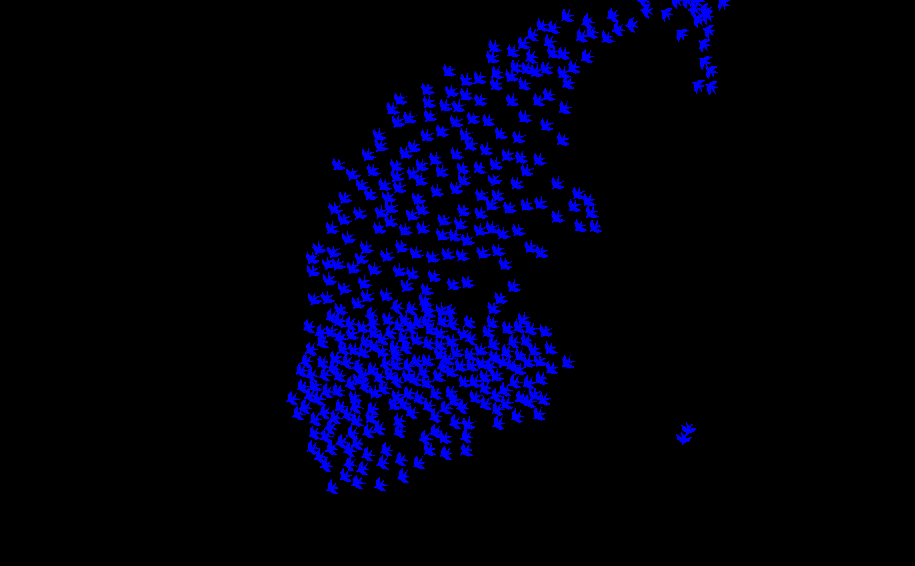
\includegraphics[width=0.7\textwidth]{../../images/boidsvisualizzationexample.png}
    \end{center}
\end{minipage}

\section{The Three Fundamental Rules}

\begin{itemize}
    \item \textbf{Alignment}: Each boid tries to match its velocity (direction and speed) to the average velocity of its local neighbors. This causes the group to move in a similar direction, promoting coordinated movement.
    \item \textbf{Cohesion}: Each boid steers towards the average position (center of mass) of its nearby flockmates. This keeps the group together and prevents individuals from straying too far from the flock.
    \item \textbf{Separation}: Each boid actively avoids crowding by steering away from neighbors that are too close. This prevents collisions and maintains a comfortable distance between individuals.
\end{itemize}

\vspace{0.5cm}
Each boid follows these rules independently, creating realistic flocking patterns without central control.

\section{Project Goals}

\begin{itemize}
    \item Implement efficient Boids simulation in C++
    \item Compare sequential vs parallel implementations
    \item Analyze different data layouts: Array of Structures (AoS) vs Structure of Arrays (SoA)
    \item Evaluate performance scalability with OpenMP
    \item Utilize SIMD optimizations where possible
\end{itemize}

\section{Implementation Overview}

\textbf{Technologies Used:}
\begin{itemize}
    \item \textbf{Language}: C++ for performance
    \item \textbf{Parallelization}: OpenMP for multi-core optimization
    \item \textbf{Visualization}: SFML (Simple and Fast Multimedia Library)
    \item \textbf{Build System}: CMake for cross-platform compilation
\end{itemize}



\chapter{Implementation Details}

\section{Data Layout Comparison: AoS vs SoA}

\subsection{Array of Structures (AoS)}
\textbf{Traditional object-oriented approach}

\begin{center}
\begin{minipage}{0.48\textwidth}
\centering
\begin{lstlisting}[style=cppstyle]
struct BoidData {
    sf::Vector2f position;
    sf::Vector2f velocity;
    float biasval;
    int scoutGroup;
};
\end{lstlisting}
\end{minipage}
\hfill
\begin{minipage}{0.48\textwidth}
\centering
\begin{itemize}
    \item Easy to understand and maintain
    \item Less cache-friendly for bulk operations
    \item Memory accesses can be scattered
\end{itemize}
\end{minipage}
\end{center}

\newpage
\subsection{Structure of Arrays (SoA)}
\textbf{Performance-optimized layout}

\begin{center}
\begin{minipage}{0.48\textwidth}
\centering
\begin{lstlisting}[style=cppstyle]
struct BoidDataList {
    float* xPos;
    float* yPos;
    float* xVelocity;
    float* yVelocity;
    float* biasvals;
    int* scoutGroup;
    int numBoid;
};
\end{lstlisting}
\end{minipage}
\hfill
\begin{minipage}{0.48\textwidth}
\centering
\begin{itemize}
    \item Better cache utilization
    \item Enables SIMD vectorization
    \item Contiguous memory access patterns
\end{itemize}
\end{minipage}
\end{center}

\section{Sequential Implementation}

\textbf{Main Algorithm Structure:}
\begin{lstlisting}[style=cppstyle]
for (int i = 0; i < num_boids; i++) {
    // Compute alignment, cohesion, separation
    for (int j = 0; j < num_boids; j++) {
        if (i != j && distance < perception_radius) {
            // Apply boid interaction rules
        }
    }
    // Update position and velocity
}
\end{lstlisting}

\textbf{Characteristics:}
\begin{itemize}
    \item O(N²) computational complexity
    \item Perfect candidate for parallelization
\end{itemize}

\section{Parallel Implementation with OpenMP}

\textbf{Key Parallelization Strategy:}
\begin{lstlisting}[style=cppstyle]
#pragma omp parallel for schedule(static)
for (int i = 0; i < N; i++) {
    // Each thread processes different boids
    // Thread-safe access to read-only data
    // Write to separate temporary arrays
}

#pragma omp simd
for (int i = 0; i < N; i++) {
    // Vectorized copy back to main arrays
    boidDataList.xPos[i] = new_xPos[i];
    boidDataList.yPos[i] = new_yPos[i];
    // ...
}
\end{lstlisting}

\textbf{Thread Safety Approach:}
\begin{itemize}
    \item Read-only access to current state
    \item Write results to temporary arrays
    \item Vectorized copy-back operation
    \item No race conditions or data dependencies
\end{itemize}

\textbf{Compiler Vectorization Enablers:}
\begin{itemize}
    \item Contiguous memory access (SoA layout)
    \item \texttt{\#pragma omp simd} directives
    \item Multiple data elements processed per instruction
\end{itemize}

\chapter{Experimental Setup}

\section{Benchmark Methodology}

\textbf{Testing Environment:}
\begin{itemize}
    \item Multi-core CPU system (12 cores)
    \item Identical simulation parameters across all tests
    \item Multiple runs per configuration for statistical accuracy (30 runs)
    \item Isolated measurement of core algorithm (no rendering overhead)
\end{itemize}

\textbf{Test Parameters:}
\begin{itemize}
    \item \textbf{Boid populations}: 1,000 to 32,000 agents
    \item \textbf{Thread configurations}: 1 to 12 threads
    \item \textbf{Implementations}: Sequential AoS vs Sequential SoA vs Parallel SoA
\end{itemize}

\section{Performance Metrics}

\textbf{Primary Measurements:}
\begin{itemize}
    \item Execution time per simulation step
    \item Speedup vs sequential baseline
    \item Scaling efficiency with thread count
\end{itemize}

\textbf{Analysis Focus:}
\begin{itemize}
    \item Impact of data layout optimization
    \item Parallel scalability characteristics  
    \item Optimal thread configuration
    \item Performance vs problem size relationship
\end{itemize}

\section{Computational Complexity Analysis}

\textbf{Algorithm Characteristics:}
\begin{itemize}
    \item \textbf{Time Complexity}: O(N²) per simulation step
    \item \textbf{Space Complexity}: O(N) for boid storage
    \item \textbf{Parallel Potential}: Embarrassingly parallel outer loop
\end{itemize}

\chapter{Performance Results}

\section{Data Layout Impact: AoS vs SoA}

\begin{figure}[h]
\centering
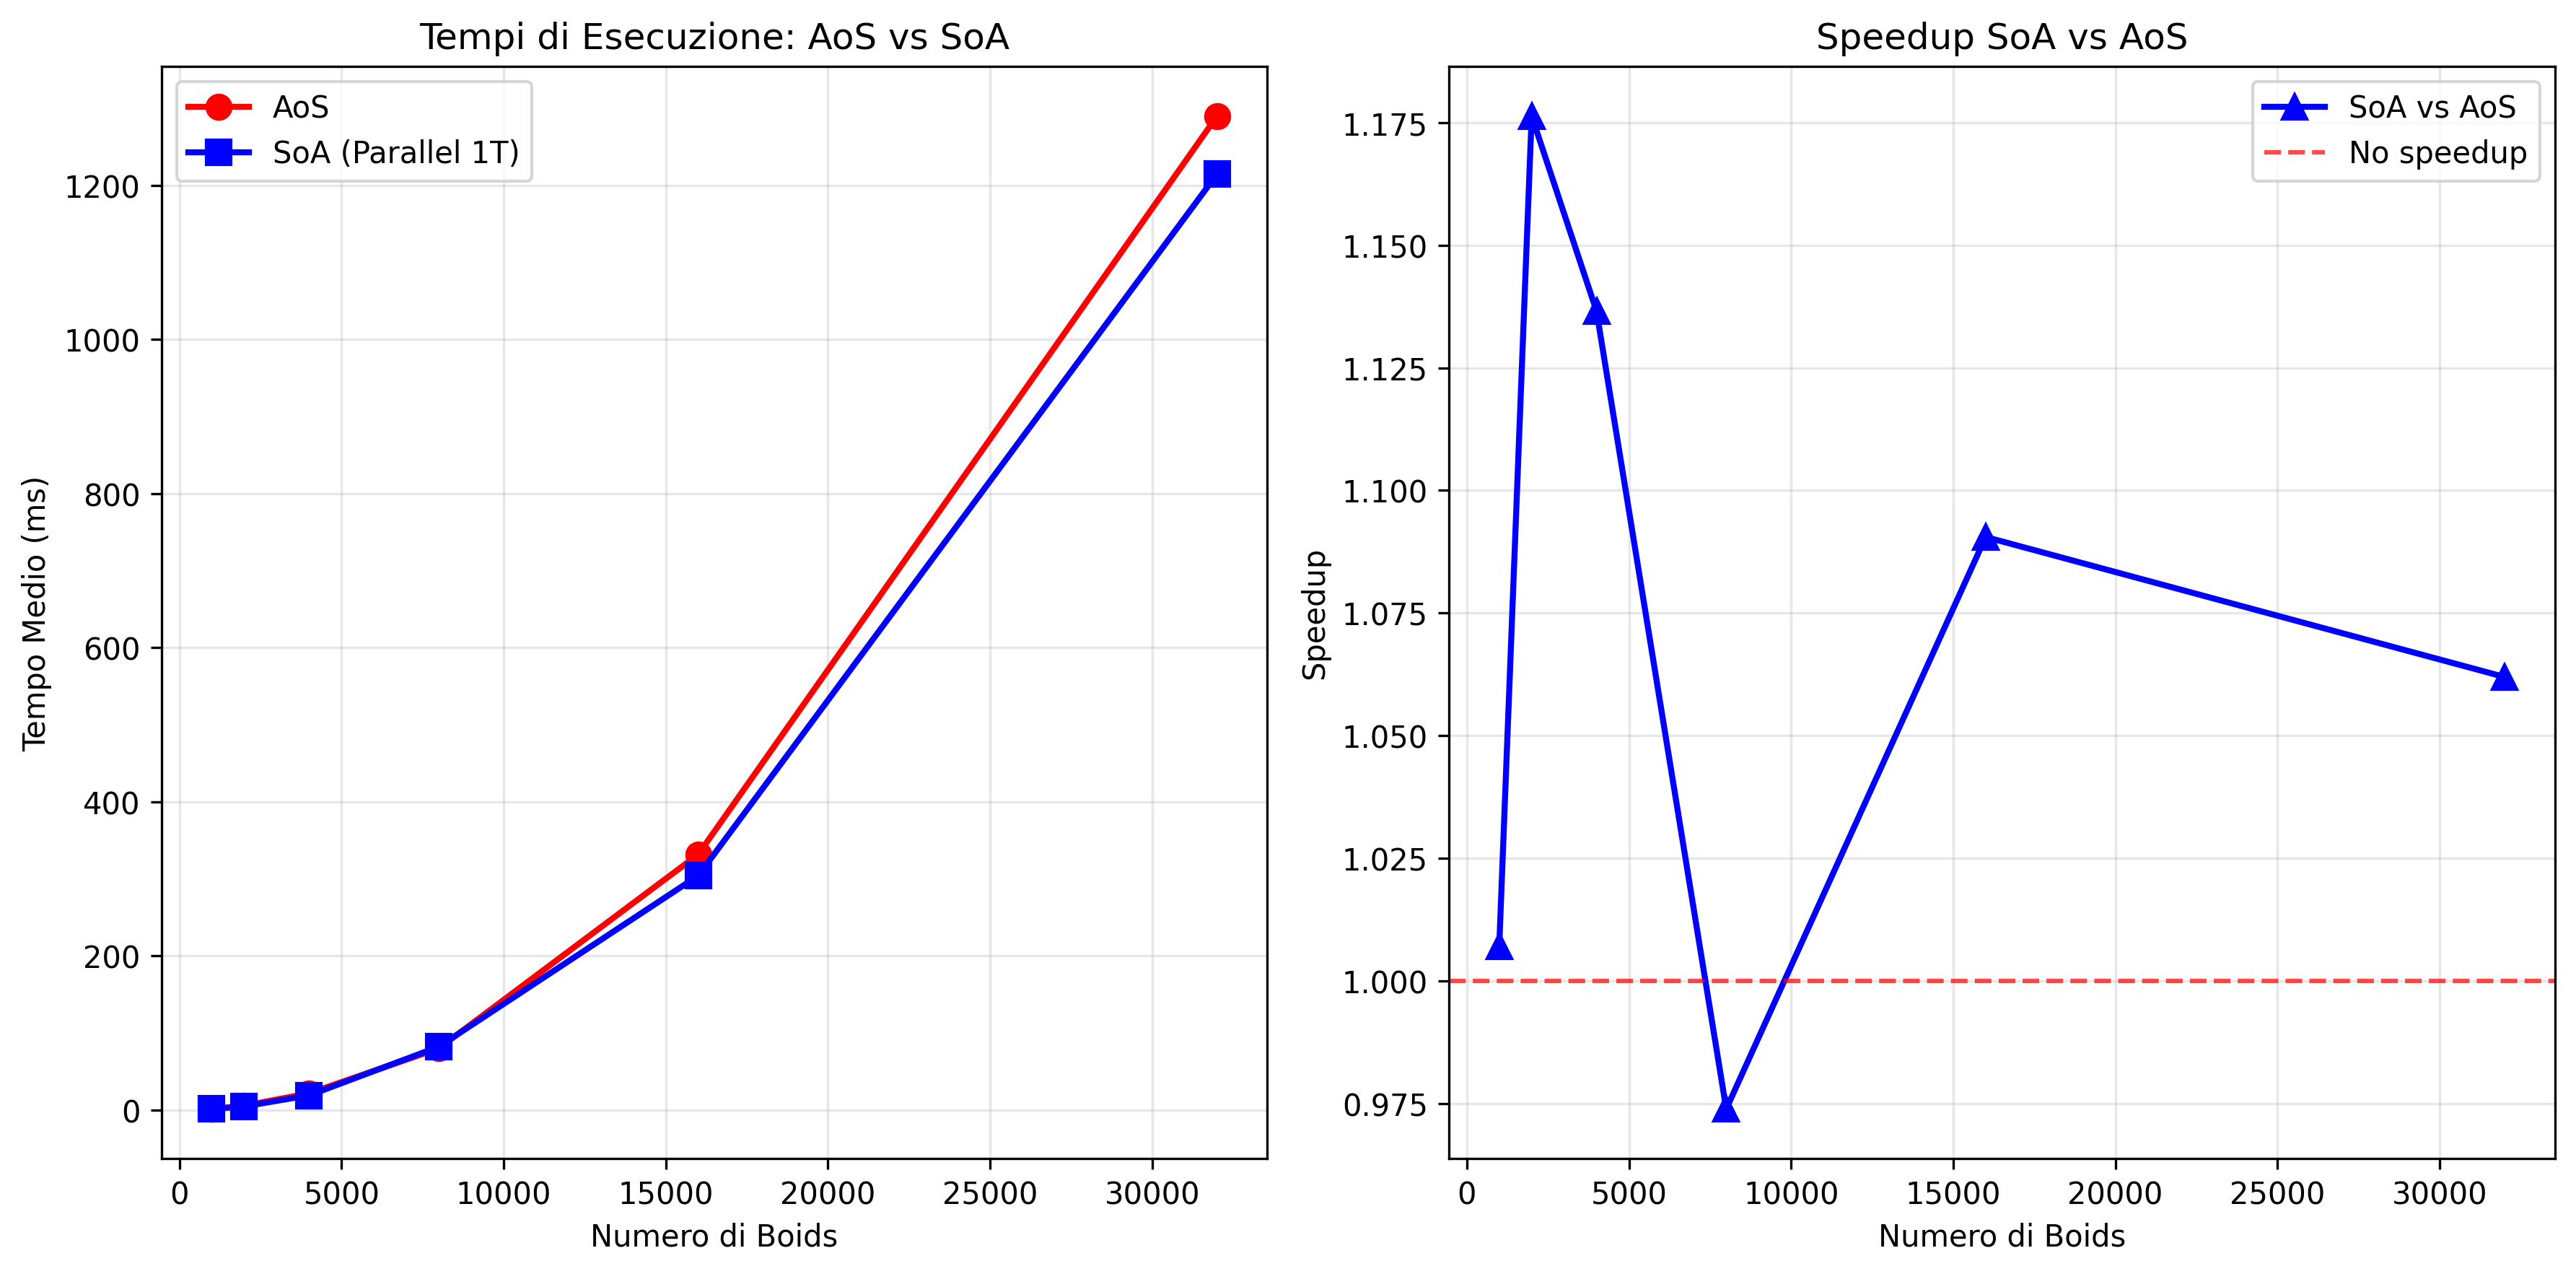
\includegraphics[width=0.95\textwidth]{../../images/aos_vs_soa.png}
\end{figure}

\textbf{Key Findings:}
\begin{itemize}
    \item SoA provides modest but consistent performance improvement
    \item 6.2\% improvement for 32,000 boids (1,290.09ms vs 1,214.82ms)
    \item Benefits become more pronounced with larger datasets
    \item Foundation for effective parallelization
\end{itemize}

\section{Parallel Scaling Performance}

\begin{figure}[h]
\centering
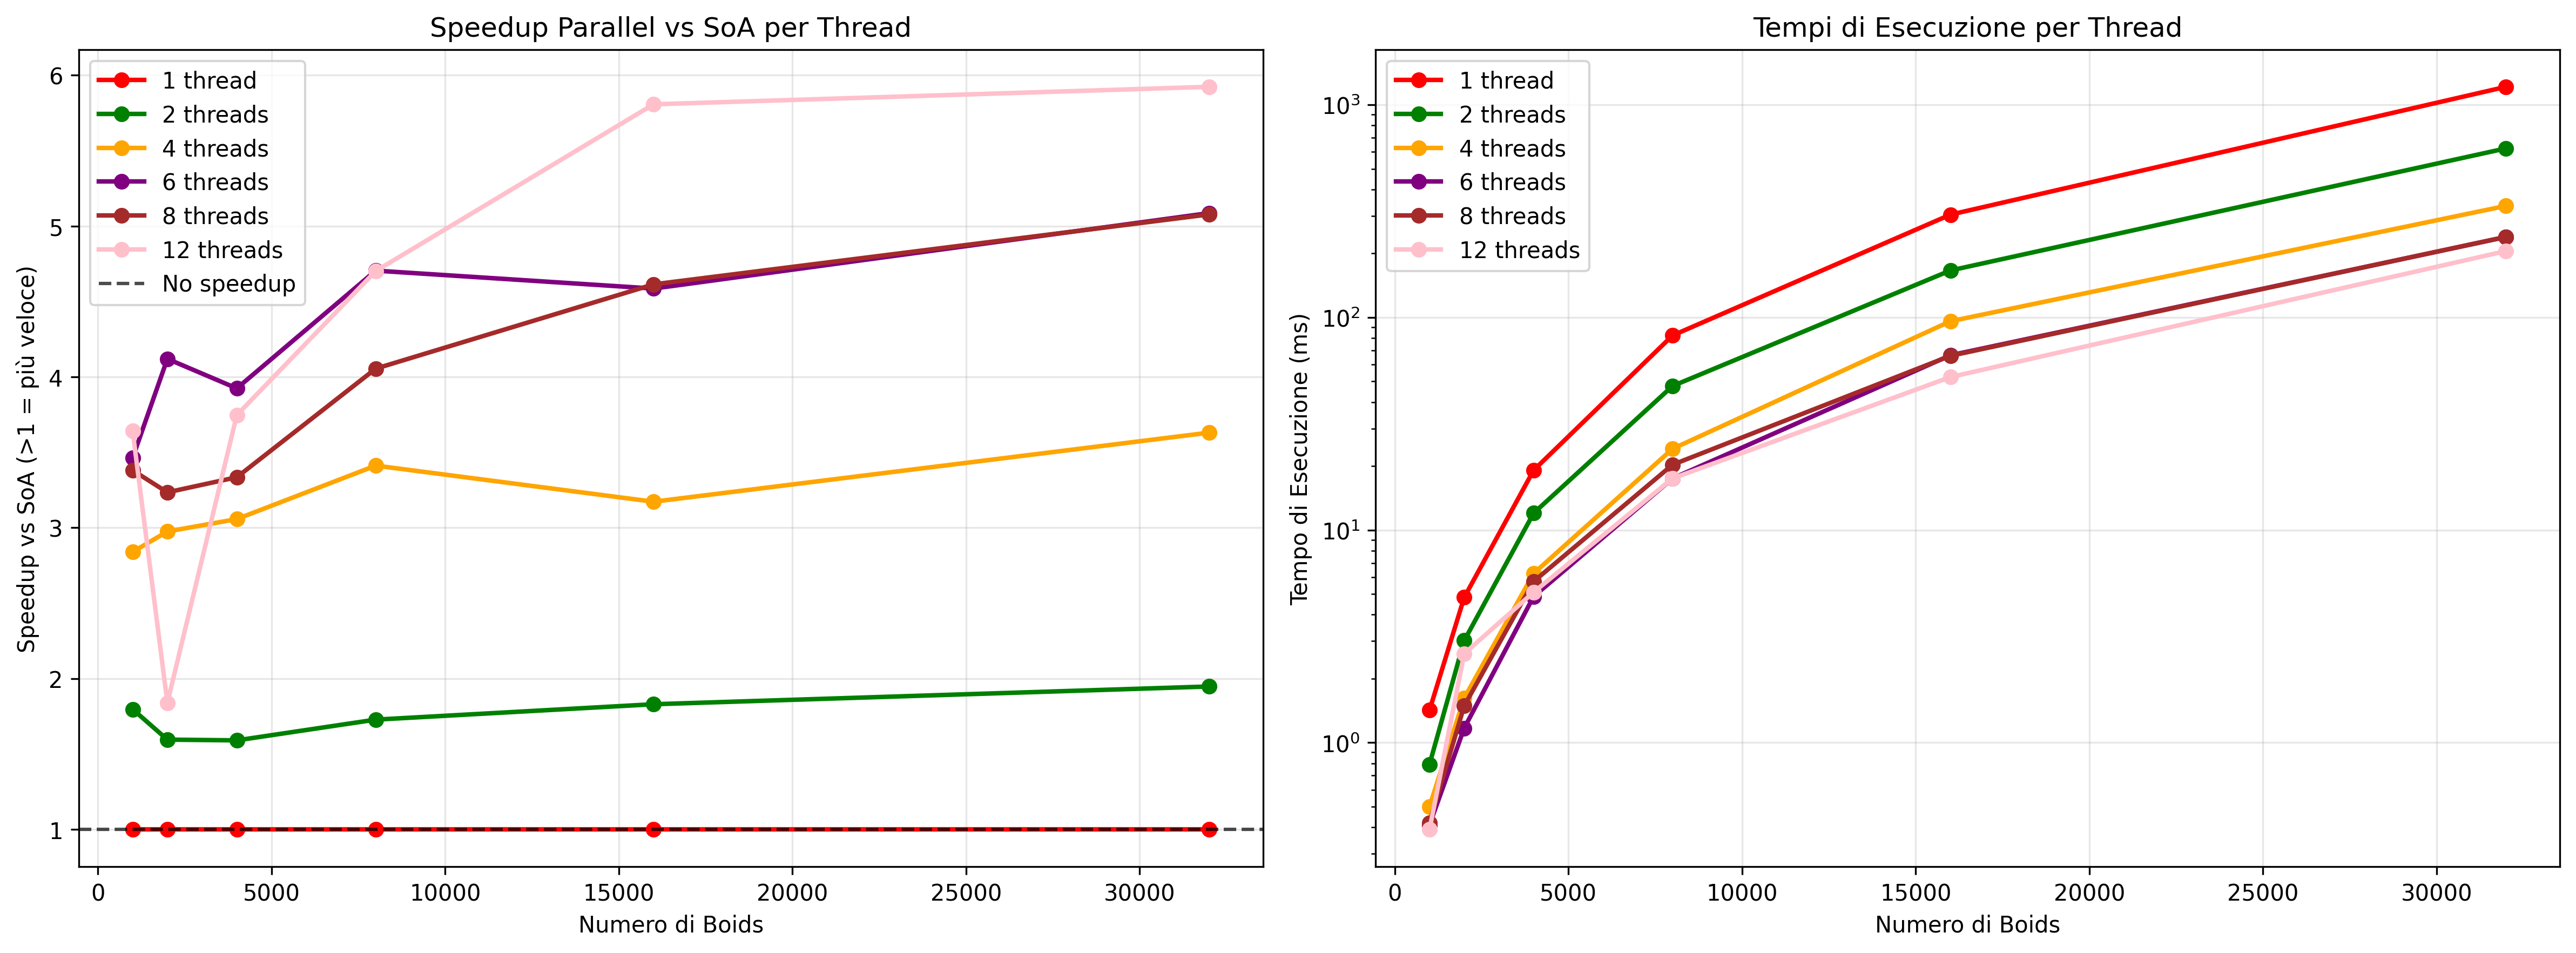
\includegraphics[width=1\textwidth]{../../images/parallel_analysis_performance.png}
\end{figure}

\newpage
\begin{center}
    \textbf{Speedup Results:}
    \begin{itemize}
        \item Near-linear scaling up to 6 threads
        \item Diminishing returns beyond 8-12 threads due to overhead
    \end{itemize}
    \begin{tabular}{|c|c|c|c|}
    \hline
    \textbf{Dataset Size} & \textbf{Sequential (ms)} & \textbf{Best Parallel (ms)} & \textbf{Speedup} \\
    \hline
    1,000 boids & 1.42 & 0.39 & 3.6x \\
    4,000 boids & 22.69 & 4.85 & 4.7x \\
    8,000 boids & 82.23 & 17.48 & 4.7x \\
    16,000 boids & 367.89 & 74.23 & 5.0x \\
    32,000 boids & 1,214.82 & 205.12 & 5.9x \\
    \hline
    \end{tabular}
\end{center}

\begin{figure}[h]
\centering
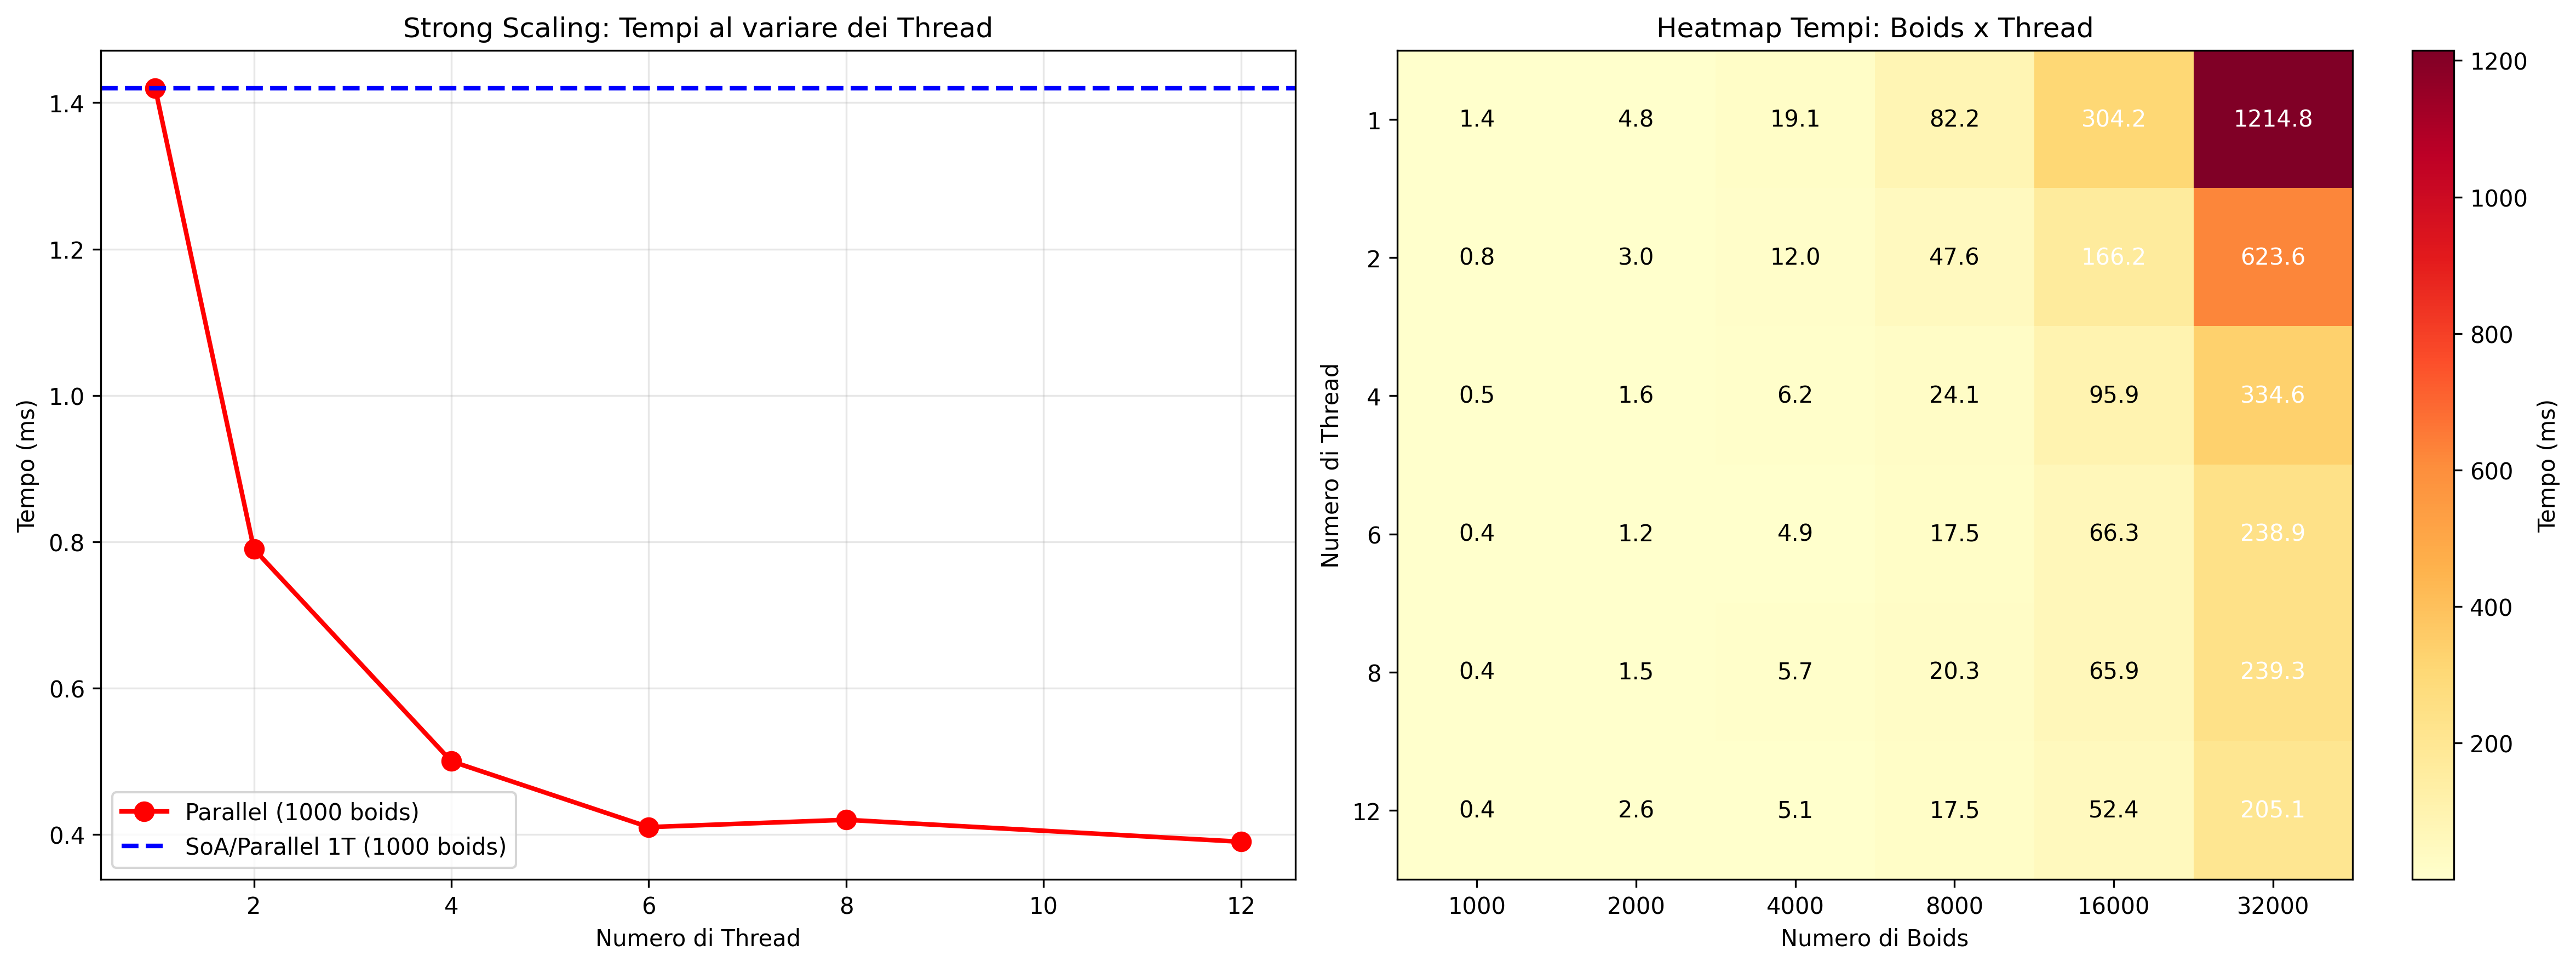
\includegraphics[width=0.95\textwidth]{../../images/parallel_analysis_scaling.png}
\end{figure}

\section{Conclusions}

\textbf{Project Achievements:}
\begin{itemize}
    \item Successfully implemented and optimized Boids simulation
    \item Demonstrated significant performance improvements through parallelization
    \item Validated importance of data structure optimization
    \item Achieved up to 5.9x speedup on multi-core systems
\end{itemize}

\chapter{Thanks for your attention
\vspace{1cm}\\
\small{Gianni Moretti}}
\end{document}
